\subsection {Unpacking raw data from the camera}
\label{sec:unpacking}


The \lucid cameras feature a 12-bit \gls{adc} and offer 23 different output formats with varying bit depths and packing.
As the \gls{h265} encoder supports up to 10-bit input, the \code{Mono10p} output format was chosen for the cameras \cite[17 ]{nvidiaNVIDIAJetsonAGX2019}
This format densly packs the 10-bit data, as depicted in Figure \ref{fig:mono10p}, maximizing the network throughput.

\begin{figure}[H]
    \centering
    \subcaptionbox{Pixel data.}{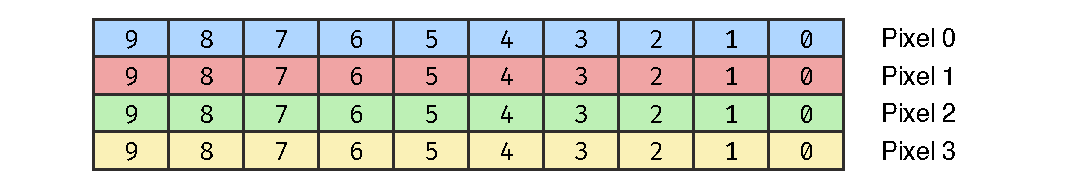
\includegraphics[width=\textwidth]{figures/unpacking/layout_10p.pdf}}
    \subcaptionbox{Bytes sent over ethernet.}{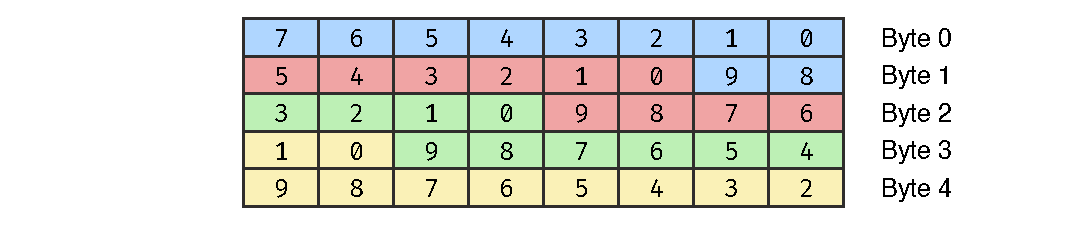
\includegraphics[width=\textwidth]{figures/unpacking/layout_10p_sent.pdf}}
    \caption{Bit layout of the \code{Mono10p} format.}
    \label{fig:mono10p}
\end{figure}


I encountered difficulties in locating documentation regarding the bit ordering on Lucid's website.
As a workaround, I relied on two test images provided by the \cam.
These test images contained pixel values that increased monotonically, as depicted in Figure \ref{fig:test_pattern}.
By analyzing the data in the first line these images, I was able to deduce the bit ordering.
Regrettably, I later discovered that Lucid Vision does provide documentation on pixel formats; however, it did not appear in their own search engine for unknown reasons \cite{lucidvisionlabsPixelFormatsLUCID2020}.

\begin{figure}[H]
    \centering
    
\includegraphics[width=0.4\textwidth]{figures/unpacking/test_pattern0.jpg}
    
\includegraphics[width=0.4\textwidth]{figures/unpacking/test_pattern2.jpg}
    \caption{Two test images used to infer the bit ordering.
        The \cam can output several different test patterns useful for various testing purposes \cite{lucidvisionlabsTritonMPPolarized2020}.}
    \label{fig:test_pattern}
\end{figure}


\subsubsection{Bit unpacking} \label{sec:contuguous_access}
The pattern in Figure \ref{fig:mono10p} was identified as being little endian, meaning the least significant bytes is stored first.


\subsubsection{Contiguous acces using warp level primitives} \label{sec:contuguous_access}
As we want to operate on 32-bit values and each pixel is stored as a 10bit value, each thread is processing 160 bits, or five words as it is the lowest common multiple of 32 and 10.
Thus every thread reads five consecutive words as shown:
\begin{align}
    a_T[i] = d[T*5+i], &  & i \in (0,1,2,3,4)
\end{align}
Where $T$ is the thread intex in the warp, $a_T$ is local memory of thread $T$, $d$ is the image stored in device memory, and $k$ is some constant offset.






It was hypothized that it would be faster to let first read the data contiguously into shared memory and then redistribute it as follows:
\begin{align}
    s[i*32+T] & = d[i*32+T],  & i & \in (0,1,2,3,4) \\
    a_T[i]    & = s[(T*5+i)], & i & \in (0,1,2,3,4)
    \label{eq:contiguous_reading}
\end{align}
Where $s$ is shared local memory of thread, but this was slower than the initial uncoalesced reading.


A secont attmempt was done using the \code{__shfl_sync} function which is a warp-level primitive used to exchange data between threads in a warp \cite{linUsingCUDAWarpLevel2018}.
As the data exchange is performed directly between registers this is faster than going through shared memory \cite{linUsingCUDAWarpLevel2018}
Data was read contiguously into local buffers of each thread, then exchanged so every thread ended up with five consecutive words.
However finding the right indices is hard as you need specity what data to send and what thread to read from, rather than what data to read from what thread.
The full index table, shown in Table \ref{table:memory_index} in Appendix \ref{chap:additional_resources}, was created and studied in order to end up with the following formulation:
\begin{align}
    c_T[i] & = d[i*32+T],       &   &                   & i & \in (0,1,2,3,4) \\
    c_T[j] & \rightarrow a_x[i] & j & = (2 * (T -i))\%5 & i & \in (0,1,2,3,4) \\
    a_T[i] & \leftarrow c_j[x]  & j & = (T*5 + i)\%32   & i & \in (0,1,2,3,4)
    \label{eq:contiguous_reading_shfl}
\end{align}
where $x$ represents the thread the data is sent to.
The code equivalent to this is written as follows.
\begin{minted}{cuda}
    a[i] = __shfl_sync(0xffffffff, c[2(*(T-i))%5], (T*5 + i)%32);
\end{minted}
